% =============================================================================
% P3A -- Privacy 2: poster (EN)
% Format: A1 portrait (594 x 841 mm), two columns, Latin Modern font.
% Expected figures in out/: Fig1_EN.pdf, Fig2_EN.pdf, Fig4_EN.pdf
% (compiled from figuras/). Content mirrors MD/P3A_Privacidade2_Poster_EN.md.
% Size tuning: \corpo (text size).
% =============================================================================
\documentclass[12pt]{article}

\usepackage[T1]{fontenc}
\usepackage[utf8]{inputenc}
\usepackage{lmodern}
\usepackage[paperwidth=594mm,paperheight=841mm,margin=18mm]{geometry}
\usepackage[brazil,english]{babel}
\usepackage{graphicx}
\usepackage{xcolor}
\usepackage[skins]{tcolorbox}
\usepackage[expansion=false]{microtype}

\pagestyle{empty}
\setlength{\parindent}{0pt}
\setlength{\parskip}{0pt}

\definecolor{exLine}{RGB}{23,54,93}
\definecolor{exFill}{RGB}{220,233,247}
\definecolor{prFill}{RGB}{200,240,236}
\definecolor{prLine}{RGB}{8,127,140}
\definecolor{prText}{RGB}{6,79,87}
\definecolor{ctxText}{RGB}{38,52,67}

\newcommand{\corpo}{\fontsize{27}{35}\selectfont}
\newcommand{\figtitulo}[1]{{\fontsize{32}{38}\selectfont\bfseries\color{exLine}#1\par}\vspace{4mm}}
\newcommand{\leitura}[1]{\vspace{4mm}{\corpo\itshape\color{ctxText}#1\par}}

\newtcolorbox{caixa}[1]{enhanced,colback=white,colframe=exLine,boxrule=1.4mm,arc=4mm,
  left=7mm,right=7mm,top=5mm,bottom=6mm,
  title={#1},fonttitle=\fontsize{34}{40}\selectfont\bfseries,coltitle=white,colbacktitle=exLine}

\begin{document}
\corpo

% ------------------------------- BANNER --------------------------------------
\begin{tcolorbox}[enhanced,colback=exLine,colframe=exLine,coltext=white,arc=4mm,
  left=12mm,right=12mm,top=9mm,bottom=9mm]
{\fontsize{58}{66}\selectfont\bfseries Privacy as a proposed PMBOK 8 performance domain\par}
\vspace{5mm}
{\fontsize{30}{38}\selectfont SIPA Privacy 2 group \ $\cdot$ \ Who (WH) concentration\par}
{\fontsize{30}{38}\selectfont\bfseries Academic proposal: processes P1--P8 are not official PMBOK 8 processes.\par}
\end{tcolorbox}

\vspace{8mm}

\noindent
\begin{minipage}[t]{0.485\linewidth}
% ------------------------------ LEFT COLUMN ----------------------------------
\begin{caixa}{Problem and contribution}
\corpo
PMBOK 8 [14] mentions data protection and privacy, but its seven domains and 40 processes do not organize personal-data processing as a separate management object. The digital-twin studies examined address legal requirements and technical controls, not project management processes [5, 11, 17]. We propose \textbf{Privacy} next to \textbf{Stakeholders (7 processes)} and \textbf{Risk (6 processes)}. Our central question is: \textbf{how might project data practices affect people, and what evidence supports the project's choices?}
\end{caixa}

\vspace{8mm}

\figtitulo{Figure 1 --- Where Privacy fits}
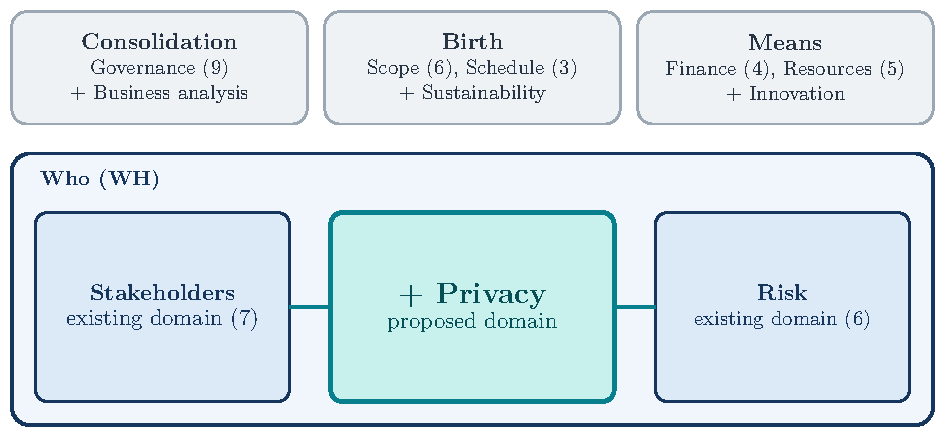
\includegraphics[width=\linewidth]{out/Fig1_EN.pdf}
\leitura{The four concentrations are an organization adopted in this work; \textbf{Privacy} is this group's contribution to the \textbf{Who} concentration.}

\vspace{8mm}

\begin{caixa}{Alignment with the 6 principles}
\corpo
\textbf{1AHV} end-to-end view of data flows\par\medskip
\textbf{2FOV} benefits weighed against potential harms\par\medskip
\textbf{3QPD} privacy as a verifiable quality criterion\par\medskip
\textbf{4BAL} accountable decisions and owners\par\medskip
\textbf{5SPA} lasting effects on people\par\medskip
\textbf{6BEC} channels for challenge and learning
\end{caixa}
\end{minipage}\hfill
\begin{minipage}[t]{0.485\linewidth}
% ------------------------------ RIGHT COLUMN ---------------------------------
\figtitulo{Figure 2 --- How the domain spans the project}
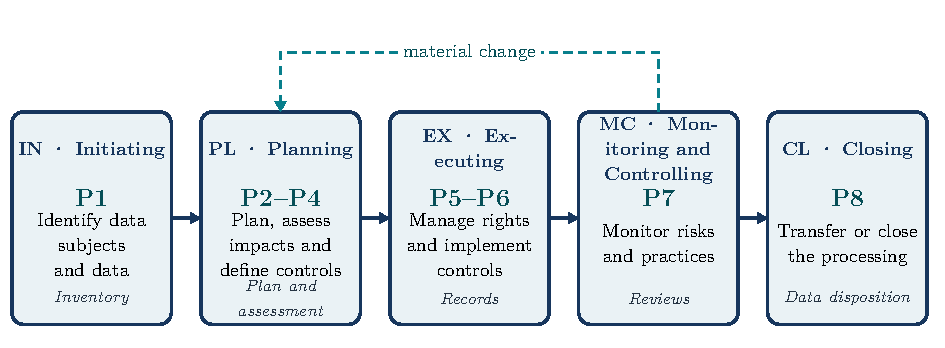
\includegraphics[width=\linewidth]{out/Fig2_EN.pdf}
\leitura{\textbf{P1--P8 are group proposals}. The return arrow represents reassessment; data processing may continue after project closure.}

\vspace{8mm}

\figtitulo{Figure 3 --- Digital twins: flow direction sets the exposure}
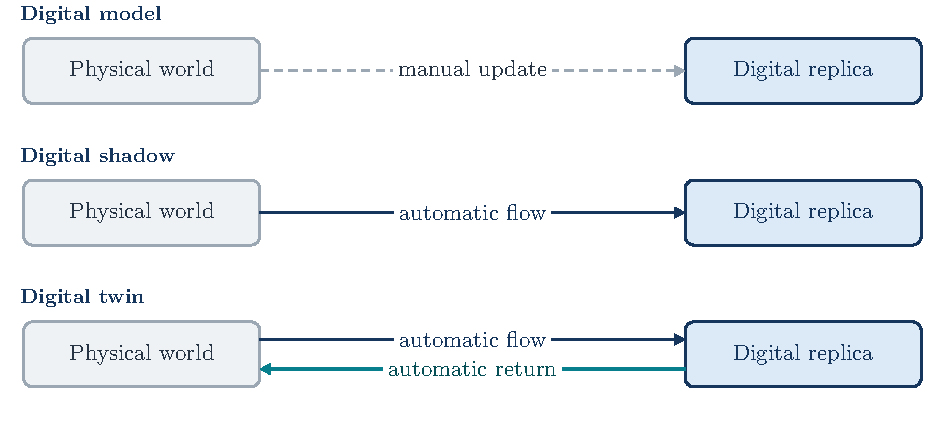
\includegraphics[width=\linewidth]{out/Fig4_EN.pdf}
\leitura{The classification follows Kritzinger et al. [12]; the more automatic and frequent the flow, the greater the exposure of people. P1--P8 should identify data subjects, purposes, sharing, risks, and data disposition without duplicating Stakeholders and Risk. The proposed inclusions in the 13 existing processes and the interfaces with the other concentrations are in the report (\S7).}

\vspace{8mm}

\begin{caixa}{References}
\fontsize{20}{26}\selectfont
Numbering of the full report, in alphabetical order.\par\smallskip
[1] ANPD. Relatório de Impacto à Proteção de Dados Pessoais (RIPD): perguntas e respostas.\par
[2] BRAZIL. Law No. 13,709/2018 (LGPD).\par
[3] BROOKS et al. NISTIR 8062, 2017.\par
[5] DHINAKARAN et al. \textit{MethodsX}, 2025.\par
[6] DTC. Digital Twin Consortium defines digital twin, 2020.\par
[7] DTC. Digital twins capabilities periodic table, v. 1.2, 2025.\par
[8] DTC. AI agent capabilities periodic table, v. 1.0, 2025.\par
[11] KORCHENKO et al. \textit{Sustainability}, 2026.\par
[12] KRITZINGER et al. \textit{IFAC-PapersOnLine}, 2018.\par
[13] NIST. Privacy Framework v. 1.0, 2020.\par
[14] PMI. \textit{PMBOK Guide}, 8th ed., 2025 (\S\S2.5 and 2.7).\par
[17] WANG et al. \textit{IEEE Internet of Things Journal}, 2023.\par\smallskip
Full references, with DOI and URL, in the report.
\end{caixa}
\end{minipage}

\end{document}
